\section{Injections}
\label{sec:appendix_injections}

This chapter describes some extra options when using our injections to integrate handwritten code with generated code. 
This complements the short introduction in Chapter~\ref{sec:intro_injections}.

As an example, we shall provide functionality for saving our \textsf{DoubleLinkedList} to a file.

\begin{enumerate}
  \item[$\blacktriangleright$] Begin with an empty workspace, create a new metamodel \textsf{Demo} and replace the \textsf{Demo.eap} with the file from our .zip file (in the folder containing this tutorial). 
  \item[$\blacktriangleright$] Now open \textsf{Demo.eap} and change the ``Default Language for Code Generation'' (Tools $\rightarrow$ Options $\rightarrow$ Source Code Engineering) to \textsf{Ecore}. 
  \item[$\blacktriangleright$] Add the method \textsf{void toFile(EString path)} to the class \textsf{List} (Fig.~\ref{fig:append_inj_diagram}) and export the project to your Eclipse workspace.
\end{enumerate}
\begin{figure}[htbp]
\begin{center}
  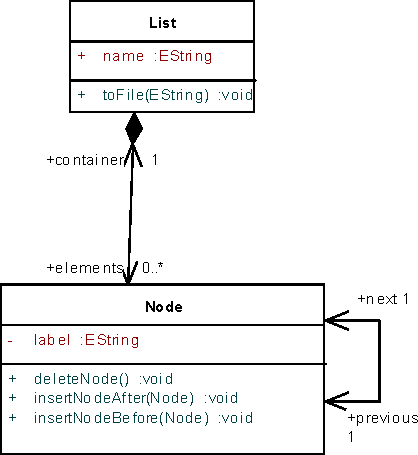
\includegraphics[width=0.5\textwidth]{pics/advancedTopics/injections/ea_diagram}
  \caption{Add a new method \textsf{toFile} to the class \textsf{List}}
  \label{fig:append_inj_diagram}
\end{center}
\end{figure}

\begin{enumerate}
  \item[$\blacktriangleright$] Implement the \textsf{toFile} method in \textsf{gen/Double\-Linked\-List\-Language/\-impl/\-ListImpl.java} with the code given in Fig. \ref{code:list_toFile_impl_code}.

\begin{figure}[htbp]
\centering
  \begin{lstlisting}[language=Java, keywordstyle={\bfseries\color{purple}}, backgroundcolor=\color{white}]
  public void toFile(String path) {
    // [user code injected with eMoflon]
    try{
      FileWriter fstream = new FileWriter(path);
      BufferedWriter out = new BufferedWriter(fstream);
      out.write(this.toText());
      out.close();
    }catch (Exception e){
      System.err.println(e.toString());
    }
  }
  \end{lstlisting}
\caption{Implementation of \texttt{toFile}}
\label{code:list_toFile_impl_code}
\end{figure}

  \item[$\blacktriangleright$] Right-click \textsf{gen/Double\-Linked\-List\-Language/\-impl/\-ListImpl.java} in the generated Eclipse project and choose ``eMoflon/create Injection for class'' to generate the file \textsf{injection/DoubleLinkedListLanguage/\-impl/List\-Impl\-.in\-ject} or update it if it already exists.
	It will contain an injection for the code given in Fig.~\ref{code:list_toFile_impl_code}.
  \item[$\blacktriangleright$] Now rebuild your project (right-click on \texttt{DoubleLinkedListLanguage} and choose ``eMoflon/Build (and clean)''). 
  This will rebuild your project and inject the code that we just wrote into \textsf{ListImpl.java}. 
  \item[$\blacktriangleright$] You will now find two additional comments just below the imports in the file. 
  To generate imports in our injection and get rid of those ``...cannot be resolved'' errors, insert the required imports between the comments as depicted in Fig. \ref{code:imports_toFile}.
\begin{figure}[htbp]
\centering
  \begin{lstlisting}[language=Java, keywordstyle={\bfseries\color{purple}}, backgroundcolor=\color{white}]
// <-- [user defined imports]
import java.io.*;
// [user defined imports] -->
  \end{lstlisting}
\caption{Imports for \texttt{toFile}}
\label{code:imports_toFile}
\end{figure}

  \item[$\blacktriangleright$] Now choose ``eMoflon/create Injection for class'' again for \textsf{ListImpl.java} to update the injection file and add the imports.

  \item[$\blacktriangleright$] To implement the missing \texttt{toText} method as a \emph{member}, insert the code between the comments at the very end of the file as depicted in Fig. \ref{code:toText_impl}

\begin{figure}[htbp]
\centering
  \begin{lstlisting}[language=Java, keywordstyle={\bfseries\color{purple}}, backgroundcolor=\color{white}]
// <-- [user code injected with eMoflon]
private String toText(){
  StringBuilder sb = new StringBuilder();
  for(Node element : elements){
    sb.append(element.getLabel());
    sb.append("\n");
  }
  return sb.toString();
}
// [user code injected with eMoflon] -->
  \end{lstlisting}
\caption{Implementation of \texttt{toText}}
\label{code:toText_impl}
\end{figure}

\end{enumerate}

In this way, member functions and fields that were \emph{not} modelled in EA can be injected using the \texttt{@members} keyword. 
Everything between \texttt{<--  -->} is copied into the end of the generated \textsf{ListImpl.java} file without any restrictions at all.

Although it is possible to also inject members in the interface file (i.e., \textsf{List.java} in this example), this is considered dirty and should be used very sparingly (if possible never).

If you ever forget what comments are required to insert imports or code for members, you can always generate an empty injection and rebuild the project to generate the required comments.

\clearpage